\documentclass[11pt,a4paper]{article}
\usepackage[a4paper,top=15mm,bottom=15mm,left=18mm,right=18mm]{geometry}
\usepackage[T1]{fontenc}
\usepackage{amsmath}
\usepackage{amssymb}
\usepackage{enumitem}
\usepackage{array}
\usepackage{xcolor}
\usepackage[most]{tcolorbox}
\usepackage{tikz}
\usetikzlibrary{arrows.meta,calc,decorations.pathreplacing}

\pagestyle{empty}
\setlength{\parindent}{0pt}
\setlength{\parskip}{4pt}

\newtcolorbox{solbox}{
  breakable,
  colback=blue!2,
  colframe=blue!40,
  boxrule=0.6pt,
  left=6pt,right=6pt,top=4pt,bottom=4pt,
  title={\bfseries Worked solution},
  colbacktitle=blue!8,
  coltitle=blue!50!black,
  fonttitle=\small
}

\begin{document}

\begin{center}
  {\Large\bfseries Worked Solutions: Reading Scales and Error Intervals}
\end{center}

\noindent
For a reading \(R\) on a scale where one gap between ticks is \(g\), half a gap is \(g/2\). The error interval is
\[
R-\frac{g}{2}\le \text{true value}<R+\frac{g}{2}.
\]
The lower bound is included, and the upper bound is not included.

\section*{Part 1: Reading a scale to the nearest tick}

\begin{enumerate}[label=\textbf{Q\arabic*.}, leftmargin=*, itemsep=8pt]

\item 
\begin{solbox}
The ticks are \(1\,\text{cm}\) apart. The pencil tip is between \(13\,\text{cm}\) and \(14\,\text{cm}\), and it is nearer to \(14\,\text{cm}\). Therefore the reading to the nearest tick is
\[
\boxed{14\,\text{cm}}.
\]
\end{solbox}

\item 
\begin{solbox}
One gap between ticks is \(1\,\text{cm}\). The door edge is at \(76.3\,\text{cm}\), which is between \(76\,\text{cm}\) and \(77\,\text{cm}\), and nearer to \(76\,\text{cm}\). Therefore the reading to the nearest tick is
\[
\boxed{76\,\text{cm}}.
\]
\end{solbox}

\item 
\begin{solbox}
One gap between ticks is \(20\,\text{ml}\). The water surface is at \(334\,\text{ml}\), which is between \(320\,\text{ml}\) and \(340\,\text{ml}\), and nearer to \(340\,\text{ml}\). Therefore
\[
\boxed{\text{one gap}=20\,\text{ml}},\qquad \boxed{\text{reading}=340\,\text{ml}}.
\]
\end{solbox}

\item 
\begin{solbox}
One gap between ticks is \(2\,\text{ml}\). The liquid surface is at \(36.6\,\text{ml}\), which is between \(36\,\text{ml}\) and \(38\,\text{ml}\), and nearer to \(36\,\text{ml}\). Therefore
\[
\boxed{\text{one gap}=2\,\text{ml}},\qquad \boxed{\text{reading}=36\,\text{ml}}.
\]
\end{solbox}

\item 
\begin{solbox}
One gap between ticks is \(10\,\text{g}\). The needle is at \(437\,\text{g}\), which is between \(430\,\text{g}\) and \(440\,\text{g}\), and nearer to \(440\,\text{g}\). Therefore
\[
\boxed{\text{one gap}=10\,\text{g}},\qquad \boxed{\text{reading}=440\,\text{g}}.
\]
\end{solbox}

\item 
\begin{solbox}
One gap between ticks is \(1\,\text{mm}=0.1\,\text{cm}\). The end of the rubber is at \(5.37\,\text{cm}\), which is between \(5.3\,\text{cm}\) and \(5.4\,\text{cm}\), and nearer to \(5.4\,\text{cm}\). Therefore
\[
\boxed{\text{one gap}=1\,\text{mm}=0.1\,\text{cm}},\qquad \boxed{\text{reading}=5.4\,\text{cm}}.
\]
\end{solbox}

\item 
\begin{solbox}
One gap between ticks is \(0.2\,\text{kg}\). The pointer is at \(23.66\,\text{kg}\), which is between \(23.6\,\text{kg}\) and \(23.8\,\text{kg}\), and nearer to \(23.6\,\text{kg}\). Therefore
\[
\boxed{\text{one gap}=0.2\,\text{kg}},\qquad \boxed{\text{reading}=23.6\,\text{kg}}.
\]
\end{solbox}

\item 
\begin{solbox}
One gap between ticks is \(0.1\,\text{m}\). The water surface is at \(1.27\,\text{m}\), which is between \(1.2\,\text{m}\) and \(1.3\,\text{m}\), and nearer to \(1.3\,\text{m}\). Therefore the reading to the nearest tick is
\[
\boxed{1.3\,\text{m}}.
\]
\end{solbox}

\end{enumerate}

\section*{Part 2: Error intervals}

\begin{enumerate}[label=\textbf{Q\arabic*.}, start=9, leftmargin=*, itemsep=8pt]

\item 
\begin{solbox}
The gap between ticks is \(1\,\text{cm}\), so half a gap is
\[
1\div 2=0.5\,\text{cm}.
\]
The reading is \(48\,\text{cm}\). Hence
\[
\text{lower bound}=48-0.5=47.5\,\text{cm},
\]
\[
\text{upper bound}=48+0.5=48.5\,\text{cm}.
\]
The upper bound is not included, so the error interval is
\[
\boxed{47.5\,\text{cm}\le \text{length}<48.5\,\text{cm}}.
\]
On a number line, draw a filled circle at \(47.5\,\text{cm}\), an open circle at \(48.5\,\text{cm}\), and shade the part between them.
\end{solbox}

\item 
\begin{solbox}
The gap between ticks is \(20\,\text{ml}\), so half a gap is
\[
20\div 2=10\,\text{ml}.
\]
The reading is \(180\,\text{ml}\). Hence
\[
\text{lower bound}=180-10=170\,\text{ml},
\]
\[
\text{upper bound}=180+10=190\,\text{ml}.
\]
The upper bound is not included, so the error interval is
\[
\boxed{170\,\text{ml}\le \text{volume}<190\,\text{ml}}.
\]
On a number line, draw a filled circle at \(170\,\text{ml}\), an open circle at \(190\,\text{ml}\), and shade the part between them.
\end{solbox}

\item 
\begin{solbox}
For each reading, subtract and add half a gap, and leave the upper bound open.
\begin{itemize}[leftmargin=*, itemsep=2pt]
\item Q1: reading \(14\,\text{cm}\), gap \(1\,\text{cm}\), half gap \(0.5\,\text{cm}\):
\[
13.5\,\text{cm}\le \text{length}<14.5\,\text{cm}.
\]
\item Q3: reading \(340\,\text{ml}\), gap \(20\,\text{ml}\), half gap \(10\,\text{ml}\):
\[
330\,\text{ml}\le \text{volume}<350\,\text{ml}.
\]
\item Q6: reading \(5.4\,\text{cm}\), gap \(0.1\,\text{cm}\), half gap \(0.05\,\text{cm}\):
\[
5.35\,\text{cm}\le \text{length}<5.45\,\text{cm}.
\]
\item Q7: reading \(23.6\,\text{kg}\), gap \(0.2\,\text{kg}\), half gap \(0.1\,\text{kg}\):
\[
23.5\,\text{kg}\le \text{mass}<23.7\,\text{kg}.
\]
\end{itemize}
\end{solbox}

\item 
\begin{solbox}
\renewcommand{\arraystretch}{1.35}
\begin{center}
\footnotesize
\setlength{\tabcolsep}{3pt}
\begin{tabular}{|>{\raggedright\arraybackslash}p{3.6cm}|c|c|c|c|>{\raggedright\arraybackslash}p{4.6cm}|}
\hline
\textbf{What is measured} & \textbf{Reading} & \textbf{Half of the gap} & \textbf{Lower bound} & \textbf{Upper bound} & \textbf{Error interval}\\
\hline
A pencil, ruler marked every \(1\,\text{cm}\) & \(15\,\text{cm}\) & \(0.5\,\text{cm}\) & \(14.5\,\text{cm}\) & \(15.5\,\text{cm}\) & \(14.5\,\text{cm}\le L<15.5\,\text{cm}\)\\
\hline
A beetle, ruler marked every \(1\,\text{mm}\) & \(23\,\text{mm}\) & \(0.5\,\text{mm}\) & \(22.5\,\text{mm}\) & \(23.5\,\text{mm}\) & \(22.5\,\text{mm}\le L<23.5\,\text{mm}\)\\
\hline
A bag of flour, scales marked every \(10\,\text{g}\) & \(510\,\text{g}\) & \(5\,\text{g}\) & \(505\,\text{g}\) & \(515\,\text{g}\) & \(505\,\text{g}\le m<515\,\text{g}\)\\
\hline
A pupil's height, chart marked every \(2\,\text{cm}\) & \(148\,\text{cm}\) & \(1\,\text{cm}\) & \(147\,\text{cm}\) & \(149\,\text{cm}\) & \(147\,\text{cm}\le h<149\,\text{cm}\)\\
\hline
Orange juice, jug marked every \(50\,\text{ml}\) & \(250\,\text{ml}\) & \(25\,\text{ml}\) & \(225\,\text{ml}\) & \(275\,\text{ml}\) & \(225\,\text{ml}\le V<275\,\text{ml}\)\\
\hline
A parcel, scales marked every \(0.2\,\text{kg}\) & \(3.4\,\text{kg}\) & \(0.1\,\text{kg}\) & \(3.3\,\text{kg}\) & \(3.5\,\text{kg}\) & \(3.3\,\text{kg}\le m<3.5\,\text{kg}\)\\
\hline
Medicine, syringe marked every \(0.5\,\text{ml}\) & \(2.5\,\text{ml}\) & \(0.25\,\text{ml}\) & \(2.25\,\text{ml}\) & \(2.75\,\text{ml}\) & \(2.25\,\text{ml}\le V<2.75\,\text{ml}\)\\
\hline
A garden, tape marked every \(10\,\text{cm}\) & \(12.4\,\text{m}\) & \(0.05\,\text{m}\) & \(12.35\,\text{m}\) & \(12.45\,\text{m}\) & \(12.35\,\text{m}\le L<12.45\,\text{m}\)\\
\hline
\end{tabular}
\end{center}
Here \(L\) denotes length, \(m\) mass, \(h\) height and \(V\) volume.
\end{solbox}

\end{enumerate}

\section*{Part 3: Using error intervals}

\begin{enumerate}[label=\textbf{Q\arabic*.}, start=13, leftmargin=*, itemsep=8pt]

\item 
\begin{solbox}
The reading is the midpoint of the error interval, and the gap is the total width of the interval.
\begin{enumerate}[label=(\alph*), leftmargin=*, itemsep=4pt]
\item
\[
30.5\,\text{cm}\le \text{length}<31.5\,\text{cm}.
\]
Reading:
\[
\frac{30.5+31.5}{2}=31\,\text{cm}.
\]
Gap:
\[
31.5-30.5=1\,\text{cm}.
\]
So the reading is \(\boxed{31\,\text{cm}}\) and the gap is \(\boxed{1\,\text{cm}}\).

\item
\[
245\,\text{g}\le \text{mass}<255\,\text{g}.
\]
Reading:
\[
\frac{245+255}{2}=250\,\text{g}.
\]
Gap:
\[
255-245=10\,\text{g}.
\]
So the reading is \(\boxed{250\,\text{g}}\) and the gap is \(\boxed{10\,\text{g}}\).

\item
\[
1.35\,\text{m}\le \text{height}<1.45\,\text{m}.
\]
Reading:
\[
\frac{1.35+1.45}{2}=1.40\,\text{m}.
\]
Gap:
\[
1.45-1.35=0.10\,\text{m}=10\,\text{cm}.
\]
So the reading is \(\boxed{1.4\,\text{m}}\) and the gap is \(\boxed{0.1\,\text{m}}\) (or \(10\,\text{cm}\)).
\end{enumerate}
\end{solbox}

\item 
\begin{solbox}
The scales are marked every \(0.2\,\text{kg}\), so half a gap is
\[
0.2\div 2=0.1\,\text{kg}.
\]
For a reading of \(23.0\,\text{kg}\), the error interval is
\[
23.0-0.1=22.9\,\text{kg}
\]
to
\[
23.0+0.1=23.1\,\text{kg},
\]
with the upper bound not included:
\[
22.9\,\text{kg}\le \text{mass}<23.1\,\text{kg}.
\]
The airline allows a mass of \(23\,\text{kg}\) or less. The interval includes masses greater than \(23\,\text{kg}\) (for example, \(23.05\,\text{kg}\)), so Leo cannot be sure that the suitcase is allowed.
\end{solbox}

\item 
\begin{solbox}
No, Sam is not right. The ruler is marked in millimetres, so one gap is
\[
1\,\text{mm}=0.1\,\text{cm}.
\]
Half a gap is \(0.05\,\text{cm}\). A reading of \(6.3\,\text{cm}\) therefore has error interval
\[
6.3-0.05=6.25\,\text{cm}
\]
to
\[
6.3+0.05=6.35\,\text{cm},
\]
with the upper bound not included:
\[
6.25\,\text{cm}\le \text{length}<6.35\,\text{cm}.
\]
The true length could be any value in this interval, so it is not exactly \(6.3\,\text{cm}\). Closer ticks make the measurement more precise, but they do not make it exact.
\end{solbox}

\item 
\begin{solbox}
\begin{enumerate}[label=(\alph*), leftmargin=*, itemsep=4pt]
\item Scales A are marked every \(10\,\text{g}\), so half a gap is \(5\,\text{g}\). A reading of \(200\,\text{g}\) gives
\[
200-5=195\,\text{g},\qquad 200+5=205\,\text{g}.
\]
Thus
\[
\boxed{195\,\text{g}\le \text{mass}<205\,\text{g}}.
\]
\item Scales B are marked every \(50\,\text{g}\), so half a gap is \(25\,\text{g}\). A reading of \(200\,\text{g}\) gives
\[
200-25=175\,\text{g},\qquad 200+25=225\,\text{g}.
\]
Thus
\[
\boxed{175\,\text{g}\le \text{mass}<225\,\text{g}}.
\]
\item The chef should use Scales A. The error interval \(195\,\text{g}\le \text{mass}<205\,\text{g}\) is exactly the recipe's allowed range. With Scales B, the true mass could be below \(195\,\text{g}\) or above \(205\,\text{g}\), so the recipe might fail.
\end{enumerate}
\end{solbox}

\item 
\begin{solbox}
The error interval is
\[
295\,\text{ml}\le \text{volume}<305\,\text{ml}.
\]
Its total width is
\[
305-295=10\,\text{ml}.
\]
This width is one gap between ticks, so the ticks must be \(10\,\text{ml}\) apart. (Equivalently, half a gap is \(5\,\text{ml}\), so one gap is \(2\times 5=10\,\text{ml}\).)

Draw ticks every \(10\,\text{ml}\), for example at \(290\,\text{ml}\), \(300\,\text{ml}\) and \(310\,\text{ml}\). The tick for \(300\,\text{ml}\) is already drawn; label at least two more, such as \(290\,\text{ml}\) and \(310\,\text{ml}\).

\smallskip
\begin{center}
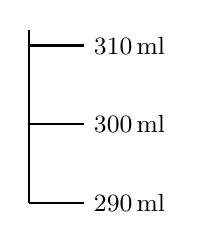
\begin{tikzpicture}[x=1cm,y=1cm]
  \draw[line width=1pt] (0,0) -- (0,2.2);
  \foreach \y/\lab in {0/290,1/300,2/310} {
    \draw[line width=0.8pt] (0,\y) -- (0.7,\y);
    \node[right,font=\small] at (0.7,\y) {\lab\,ml};
  }
\end{tikzpicture}
\end{center}
\end{solbox}

\item 
\begin{solbox}
No, the shelf will not definitely fit.

For a reading of \(80\,\text{cm}\) on a metre rule marked in centimetres, one gap is \(1\,\text{cm}\), so half a gap is \(0.5\,\text{cm}\). The error interval is
\[
80-0.5=79.5\,\text{cm}
\]
to
\[
80+0.5=80.5\,\text{cm},
\]
with the upper bound not included:
\[
79.5\,\text{cm}\le \text{length}<80.5\,\text{cm}.
\]
Both the shelf and the gap between the walls have this same error interval. It is possible that the shelf is near the top of its interval, say \(80.4\,\text{cm}\), and the gap is near the bottom, say \(79.6\,\text{cm}\). Then the shelf would not fit. To guarantee that it fits, we would need the lower bound of the gap to be greater than the upper bound of the shelf, which we do not know here.
\end{solbox}

\item 
\begin{solbox}
\textbf{Example response.}
\begin{enumerate}[label=(\alph*), leftmargin=*, itemsep=4pt]
\item I choose a kitchen measuring jug. The ticks on its scale are every \(50\,\text{ml}\).
\item A reading on this jug is \(250\,\text{ml}\). The gap is \(50\,\text{ml}\), so half a gap is \(25\,\text{ml}\). The error interval is
\[
250-25=225\,\text{ml}
\]
to
\[
250+25=275\,\text{ml},
\]
with the upper bound not included:
\[
\boxed{225\,\text{ml}\le \text{volume}<275\,\text{ml}}.
\]
\item This jug is accurate enough for making soup or a drink, where a small error of up to \(25\,\text{ml}\) does not matter. It is not accurate enough for measuring medicine, because an error of up to \(25\,\text{ml}\) could change the dose significantly.
\end{enumerate}
\end{solbox}

\end{enumerate}

\end{document}